
\newpage
\section{Analízis}
\subsection{a) Átviteli függvények}
Veszem bemenetnek a kapocsfeszültséget és a lassító $M_t$ terhelő nyomatékot, kimenetnek a tárcsa szögsebességét és az armatúraáramot. A korábban meghatározott redukált hálózat segítségével az átviteli függvények analitikusan is felírhatók (a szuperpozíció elvét alkalmazva).
\begin{itemize}
    \item \textbf{Feszültség -- szögsebesség átvitel ($M_t = 0$):} A feszültségosztó elve alapján a szögsebesség a párhuzamos $Z_e$ impedancián esik (skálázva a négypólus áttételeivel): $W_1(s) = \frac{\Omega_t}{U} = \frac{Z_e}{(Z_{12} + Z_e) k_m N}$
    \item \textbf{Feszültség -- áram átvitel ($M_t = 0$):} Az Ohm-törvény alapján az eredő impedancia reciprokaként kapjuk (figyelembe véve az áttételeket): $W_2(s) = \frac{I}{U} = \frac{1}{(Z_{12} + Z_e) k_m^2 N^2}$
    \item \textbf{Terhelőnyomaték -- szögsebesség átvitel ($U = 0$):} A terhelőnyomaték áramosztóként a két párhuzamos ágon (elektromos és mechanikai impedanciák) oszlik meg: $W_3(s) = \frac{\Omega_t}{M_t} = -\frac{Z_e Z_{12}}{Z_e + Z_{12}}$
    \item \textbf{Terhelőnyomaték -- áram átvitel ($U = 0$):} $W_4(s) = \frac{I}{M_t} = \frac{Z_e}{(Z_e + Z_{12}) k_m N}$
\end{itemize}

A behelyettesítés és egyszerűsítés után a 4 átviteli függvény:
\begin{align}
    W_1(s) & = \frac{7.2581}{7.847 \cdot 10^{-5} s^{2} + 0.7889 s + 53.9315}              \\
    W_2(s) & = \frac{0.0413 s + 0.0655}{7.847 \cdot 10^{-5} s^{2} + 0.7889 s + 53.9315}          \\
    W_3(s) & = \frac{- 0.0019 s - 19.1}{7.847 \cdot 10^{-5} s^{2} + 0.7889 s + 53.9315} \\
    W_4(s) & = \frac{7.2581}{7.847 \cdot 10^{-5} s^{2} + 0.7889 s + 53.9315}
\end{align}

\subsection{b) Állandósult értékek (statikus erősítések)}
A rendszer statikus átviteli tényezői (állandósult állapothoz tartozó erősítései) a végérték tétel alapján határozhatók meg. Állandósult állapotban egy tetszőleges konstans bemenetre (amelynek Laplace-transzformáltja $U(s) = U_0/s$) adott válasz végértéke: $\lim_{t \to \infty} y(t) = \lim_{s \to 0} s \cdot Y(s) = \lim_{s \to 0} s \cdot W(s) \frac{U_0}{s} = U_0 \lim_{s \to 0} W(s)$.
Tehát a rendszer statikus erősítése $K = W(0)$. Ezt felírva a 4 átviteli függvényre:
\begin{align}
    K_1 = \lim_{s \to 0} W_1(s) & = 0.13458 \text{ rad/s/V}   \\
    K_2 = \lim_{s \to 0} W_2(s) & = 0.001215 \text{ A/V}      \\
    K_3 = \lim_{s \to 0} W_3(s) & = -0.35415 \text{ rad/s/Nm} \\
    K_4 = \lim_{s \to 0} W_4(s) & = 0.13458 \text{ A/Nm}
\end{align}

\subsection{c) Feszültség-szögsebesség átmeneti függvénye algebrai alakban}
Az átviteli függvény polinom (algebrai) alakja a számláló és nevező polinomok hányadosaként írható fel:
\begin{equation}
    W_1(s) = \frac{b_0}{a_2 s^2 + a_1 s + a_0} = \frac{7.2581}{7.847 \cdot 10^{-5} s^{2} + 0.7889 s + 53.9315}
\end{equation}

Ebből a rendszer átmeneti függvénye (egységugrásra adott válasza) a $Y_1(s) = \frac{W_1(s)}{s}$ kifejezés inverz Laplace-transzformáltjaként adódik:
\begin{equation}
    y_1(t) = 7.2581 \cdot 10^0 \cdot e^{-5027 t} \cdot \left( A e^{4958 t} + B e^{-4958 t} \right) + 0.13458
\end{equation}
amely leegyszerűsítve az időállandókat használva ($T_1 \approx 0.01453$ s és $T_2 \approx 0.0001$ s):
\begin{equation}
    y_1(t) = 0.13458 + c_1 e^{-t/T_1} + c_2 e^{-t/T_2}
\end{equation}

\newpage
\subsection{d) Szögsebesség időfüggvénye névleges feszültség esetén}
Az alábbi ábra a szimulált görbét mutatja névleges ($u_n = 30$ V) feszültségugrásra. A végső elért szögsebesség $\approx 4.037$ rad/s.
\begin{figure}[H]
    \centering
    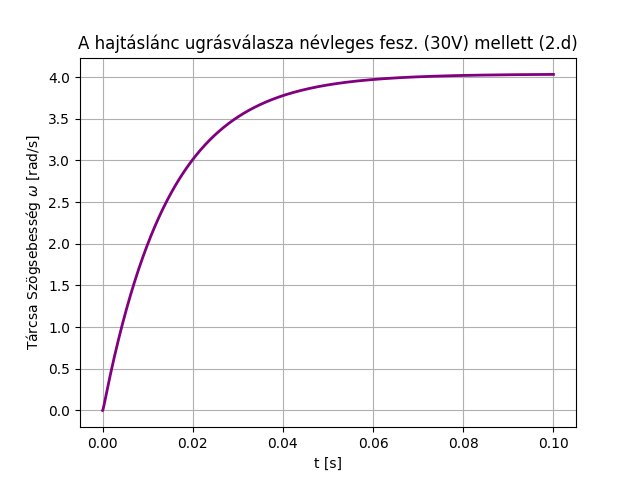
\includegraphics[width=0.8\textwidth]{res/imgs/fig_HajtaslancUgras30V.png}
    \caption{A $W_1(s)$ átviteli függvény ugrásválasza névleges feszültség (30 V) mellett}
\end{figure}

\subsection{e) Maximális terhelőnyomaték maximális áramhoz}
Tudom, hogy az áram kifejezhető a bemenetekből:
\begin{equation}
    i(t \to \infty) = W_2(0) u_n + W_4(0) M_t
\end{equation}
A maximális állandósult áram az adatlapon $0.47$ A. Ebből a terhelőnyomaték kifejezhető:
\begin{equation}
    M_t = \frac{i_{max} - W_2(0) u_n}{W_4(0)} = \frac{0.47 - 0.001215 \cdot 30}{0.13458} = 3.2215 \text{ Nm}
\end{equation}
